
%%%%%%%%%%%%%%%%%%%%%%%%%%%%%%%%%%%%%%%%%
% Programming/Coding Assignment
% LaTeX Template
%
% This template has been downloaded from:
% http://www.latextemplates.com
%
% Original author:
% Ted Pavlic (http://www.tedpavlic.com)
%
% Note:
% The \lipsum[#] commands throughout this template generate dummy text
% to fill the template out. These commands should all be removed when 
% writing assignment content.
%
% This template uses a Perl script as an example snippet of code, most other
% languages are also usable. Configure them in the "CODE INCLUSION 
% CONFIGURATION" section.
%
%%%%%%%%%%%%%%%%%%%%%%%%%%%%%%%%%%%%%%%%%

%----------------------------------------------------------------------------------------
%	PACKAGES AND OTHER DOCUMENT CONFIGURATIONS
%----------------------------------------------------------------------------------------



\documentclass{article}

\usepackage{fancyhdr} % Required for custom headers
\usepackage{lastpage} % Required to determine the last page for the footer
\usepackage{extramarks} % Required for headers and footers
\usepackage[usenames,dvipsnames]{color} % Required for custom colors
\usepackage{graphicx} % Required to insert images
\usepackage{listings} % Required for insertion of code
\usepackage{courier} % Required for the courier font
\usepackage{lipsum} % Used for inserting dummy 'Lorem ipsum' text into the template
\usepackage{setspace}
\usepackage{color}
\usepackage{comment}
\usepackage{caption}
\usepackage[T1]{fontenc}
\usepackage{hyperref}
\usepackage{natbib}
\usepackage{underscore}
\usepackage{subfigure}
\usepackage{fixltx2e}

\hypersetup{
    colorlinks=true,
    linkcolor=blue,
    filecolor=magenta,      
    urlcolor=cyan,
    breaklinks=true
}

\usepackage[]{algorithm2e}
\usepackage{pdfpages}
\usepackage{tikz}




%For python inclusion (http://widerin.org/blog/syntax-highlighting-for-python-scripts-in-latex-documents)
\definecolor{Code}{rgb}{0,0,0}
\definecolor{Decorators}{rgb}{0.5,0.5,0.5}
\definecolor{Numbers}{rgb}{0.5,0,0}
\definecolor{MatchingBrackets}{rgb}{0.25,0.5,0.5}
\definecolor{Keywords}{rgb}{0,0,1}
\definecolor{self}{rgb}{0,0,0}
\definecolor{Strings}{rgb}{0,0.63,0}
\definecolor{Comments}{rgb}{0,0.63,1}
\definecolor{Backquotes}{rgb}{0,0,0}
\definecolor{Classname}{rgb}{0,0,0}
\definecolor{FunctionName}{rgb}{0,0,0}
\definecolor{Operators}{rgb}{0,0,0}
\definecolor{Background}{rgb}{0.98,0.98,0.98}

% Margins
\topmargin=-0.45in
\evensidemargin=0in
\oddsidemargin=0in
\textwidth=6.5in
\textheight=9.0in
\headsep=0.25in

\linespread{1.1} % Line spacing

% Set up the header and footer
\pagestyle{fancy}
\lhead{\hmwkAuthorName} % Top left header
\chead{\hmwkClass\ (\hmwkClassInstructor\ \hmwkClassTime): \hmwkTitle} % Top center head
\chead{\hmwkClass\ (\hmwkClassInstructor): \hmwkTitle} % Top center head
\rhead{\firstxmark} % Top right header
\lfoot{\lastxmark} % Bottom left footer
\cfoot{} % Bottom center footer
\rfoot{Page\ \thepage\ of\ \protect\pageref{LastPage}} % Bottom right footer
\renewcommand\headrulewidth{0.4pt} % Size of the header rule
\renewcommand\footrulewidth{0.4pt} % Size of the footer rule

\setlength\parindent{0pt} % Removes all indentation from paragraphs

%----------------------------------------------------------------------------------------
%	CODE INCLUSION CONFIGURATION
%----------------------------------------------------------------------------------------

\definecolor{MyDarkGreen}{rgb}{0.0,0.4,0.0} % This is the color used for comments
\lstloadlanguages{Perl} % Load Perl syntax for listings, for a list of other languages supported see: ftp://ftp.tex.ac.uk/tex-archive/macros/latex/contrib/listings/listings.pdf
\lstset{language=Perl, % Use Perl in this example
        frame=single, % Single frame around code
        basicstyle=\small\ttfamily, % Use small true type font
        keywordstyle=[1]\color{Blue}\bf, % Perl functions bold and blue
        keywordstyle=[2]\color{Purple}, % Perl function arguments purple
        keywordstyle=[3]\color{Blue}\underbar, % Custom functions underlined and blue
        identifierstyle=, % Nothing special about identifiers                                         
        commentstyle=\usefont{T1}{pcr}{m}{sl}\color{MyDarkGreen}\small, % Comments small dark green courier font
        stringstyle=\color{Purple}, % Strings are purple
        showstringspaces=false, % Don't put marks in string spaces
        tabsize=5, % 5 spaces per tab
        %
        % Put standard Perl functions not included in the default language here
        morekeywords={rand},
        %
        % Put Perl function parameters here
        morekeywords=[2]{on, off, interp},
        %
        % Put user defined functions here
        morekeywords=[3]{test},
       	%
        morecomment=[l][\color{Blue}]{...}, % Line continuation (...) like blue comment
        numbers=left, % Line numbers on left
        firstnumber=1, % Line numbers start with line 1
        numberstyle=\tiny\color{Blue}, % Line numbers are blue and small
        stepnumber=5 % Line numbers go in steps of 5
}

% Creates a new command to include a perl script, the first parameter is the filename of the script (without .pl), the second parameter is the caption
\newcommand{\perlscript}[2]{
\begin{itemize}
\item[]\lstinputlisting[caption=#2,label=#1]{#1.pl}
\end{itemize}
}


%----------------------------------------------------------------------------------------
%	DOCUMENT STRUCTURE COMMANDS
%	Skip this unless you know what you're doing
%----------------------------------------------------------------------------------------

% Header and footer for when a page split occurs within a problem environment
\newcommand{\enterProblemHeader}[1]{
\nobreak\extramarks{#1}{#1 continued on next page\ldots}\nobreak
\nobreak\extramarks{#1 (continued)}{#1 continued on next page\ldots}\nobreak
}

% Header and footer for when a page split occurs between problem environments
\newcommand{\exitProblemHeader}[1]{
\nobreak\extramarks{#1 (continued)}{#1 continued on next page\ldots}\nobreak
\nobreak\extramarks{#1}{}\nobreak
}

\setcounter{secnumdepth}{0} % Removes default section numbers
\newcounter{homeworkProblemCounter} % Creates a counter to keep track of the number of problems

\newcommand{\homeworkProblemName}{}
\newenvironment{homeworkProblem}[1][Problem \arabic{homeworkProblemCounter}]{ % Makes a new environment called homeworkProblem which takes 1 argument (custom name) but the default is "Problem #"
\stepcounter{homeworkProblemCounter} % Increase counter for number of problems
\renewcommand{\homeworkProblemName}{#1} % Assign \homeworkProblemName the name of the problem
\section{\homeworkProblemName} % Make a section in the document with the custom problem count
\enterProblemHeader{\homeworkProblemName} % Header and footer within the environment
}{
\exitProblemHeader{\homeworkProblemName} % Header and footer after the environment
}

\newcommand{\problemAnswer}[1]{ % Defines the problem answer command with the content as the only argument
\noindent\framebox[\columnwidth][c]{\begin{minipage}{0.98\columnwidth}#1\end{minipage}} % Makes the box around the problem answer and puts the content inside
}

\newcommand{\homeworkSectionName}{}
\newenvironment{homeworkSection}[1]{ % New environment for sections within homework problems, takes 1 argument - the name of the section
\renewcommand{\homeworkSectionName}{#1} % Assign \homeworkSectionName to the name of the section from the environment argument
\subsection{\homeworkSectionName} % Make a subsection with the custom name of the subsection
\enterProblemHeader{\homeworkProblemName\ [\homeworkSectionName]} % Header and footer within the environment
}{
\enterProblemHeader{\homeworkProblemName} % Header and footer after the environment
}

%----------------------------------------------------------------------------------------
%	NAME AND CLASS SECTION
%----------------------------------------------------------------------------------------

\newcommand{\hmwkTitle}{Assignment\ \#4 } % Assignment title
%\newcommand{\hmwkDueDate}{Saturday,\ March\ 16,\ 2019} % Due date
\newcommand{\hmwkClass}{Web Science} % Course/class
%\newcommand{\hmwkClassTime}{10:30am} % Class/lecture time
\newcommand{\hmwkClassInstructor}{Alexander Nwala} % Teacher/lecturer
\newcommand{\hmwkAuthorName}{Apurva Modi} % Your name

%----------------------------------------------------------------------------------------
%	TITLE PAGE
%----------------------------------------------------------------------------------------

\title{
\vspace{2in}
\textmd{\textbf{\hmwkClass:\ \hmwkTitle}}\\
%\normalsize\vspace{0.1in}\small{Due\ on\ \hmwkDueDate}\\
%\vspace{0.1in}\large{\textit{\hmwkClassInstructor\ \hmwkClassTime}}
\vspace{0.1in}\large{\textit{\hmwkClassInstructor}}
\vspace{3in}
}

\author{\textbf{\hmwkAuthorName}}
\date{Saturday, March 16, 2019} % Insert date here if you want it to appear below your name

%----------------------------------------------------------------------------------------

\begin{document}

\maketitle
\newpage



%----------------------------------------------------------------------------------------
%	TABLE OF CONTENTS
%----------------------------------------------------------------------------------------

%\setcounter{tocdepth}{1} % Uncomment this line if you don't want subsections listed in the ToC

\newpage
\tableofcontents
\newpage

%----------------------------------------------------------------------------------------
%	PROBLEM 1
%----------------------------------------------------------------------------------------

% To have just one problem per page, simply put a \clearpage after each problem

\begin{homeworkProblem}

Determine if the friendship paradox holds for my Facebook account.* Compute the mean, median and standard deviation of the number of friends that my friends have.
Create a graph of the number of friends (y-axis) and the friends themselves, sorted by number of friends (y-axis).\\  

%\problemAnswer{
 \textbf{SOLUTION :}\\
 
  \begin{enumerate}
  \item\textbf{} To Compute Mean
  			\begin{verbatim}
				Mean = Sum of all the Friend's friend Count / Total Friend Count
			\end{verbatim}
			
			
\item\textbf{} To compute Median 
  	        		\begin{verbatim}
				Median = 	Middle Item of the Sorted Friends count
			\end{verbatim}
			
\item\textbf{} To compute Standard Deviation
  	        		\begin{verbatim}
			Standard Deviation = SquareRoot {Sum of all([Square(friend count - Mean)])
			/Total Friend Count}
			\end{verbatim}				      
 \end{enumerate}
 
 
%}
  
\begin{lstlisting}[language=Python, caption=Assignmnent4_1.py]
 #This is a Python2 Program 
import csv
import math
from astropy.table import Table
import numpy as np

friend_Dict= {}
total_Count = 0
friend_List = []
friend_Count = 0
friend_Mean = 0
friend_Median = 0
friend_SD = 0
count=1
friend_count = 0
def mean():
	global friend_Mean
	friend_Mean = round((total_Count / friend_Count),2)
	return friend_Mean

def median():
	global friend_Median
	
	mid = 0
	friend_List.sort(key=int)

	mid = len(friend_List) / 2
	if(mid == 0):
		friend_Median = friend_List[mid]
	else:
		mid = mid +1	
		friend_Median = friend_List[mid]
	return friend_Median

def SD():
	global friend_SD
	global friend_Mean
	SD_Sum = 0
	for num in friend_List:
		SD_Sum = SD_Sum + ((int(num) - int(friend_Mean)) 
						*  (int(num) - int(friend_Mean)))

	#print('SD_Sum',SD_Sum)

	friend_SD = round(math.sqrt(SD_Sum / friend_Count),2)
	return friend_SD

with open('acnwala-friendscount.csv') as csvfile:
	total_Count = 0
	readCSV = csv.reader(csvfile, delimiter=',')
	for row in readCSV:
		if  "FRIENDCOUNT" in row[1]:
			continue
		else:
			friend_List.append(row[1])
			total_Count = total_Count + int(row[1])
			friend_Count = friend_Count + 1
	print (total_Count)

friend_List.sort(key=int)
f = open('fb-Friends.txt','w')
for num in friend_List:
	print (num)
	f.write(str(count)+","+str(num))
	f.write('\n')
	count = count + 1
	friend_count = friend_count + int(num)
f.close()  
	
mean = [str(mean())]
median = [str(median())]
SD = [str(SD())]
tableList = Table([mean, median, SD], names=('MEAN', 'MEDIAN', 'STANDARD DEVIATION'))
print (tableList)
\end{lstlisting}
\newpage

\begin{lstlisting}[language=Python, caption=graph4_1.py]
 #This is a Python2 Program 

import matplotlib.pyplot as plt
import csv

x = []
y = []

with open('fb-Friends.txt','r') as csvfile:
    plots = csv.reader(csvfile, delimiter=',')
    for row in plots:
        x.append(int(row[0]))
        y.append(int(row[1]))

plt.plot(x,y)

plt.plot(11,98,marker=".", color='red',markersize=12)
plt.annotate('Dr. Nwala\'s Friends : 98' , xy=(17, 98))

plt.plot(52,431,marker=".", color='red',markersize=12)
plt.annotate('Median : 431' , xy=(40, 500))

plt.plot(63,536.67,marker=".", color='red',markersize=12)
plt.annotate('Standard Deviation : 536.67' , xy=(63, 350),)

plt.plot(65,542,marker=".", color='red',markersize=12)
plt.annotate('Mean : 542' , xy=(65, 700))

plt.xlim(0, 105)
plt.xlabel('Facebook Friends')

plt.ylabel('No. of Friends for Each Friend')
plt.title('Facebook Friends Vs Each Friend count')
plt.legend()
plt.show()

\end{lstlisting}

The below plot will show the friendship paradox for \textbf{Dr.Alexander Nwala's}  facebook account

\begin{figure}[h]
  \centering
    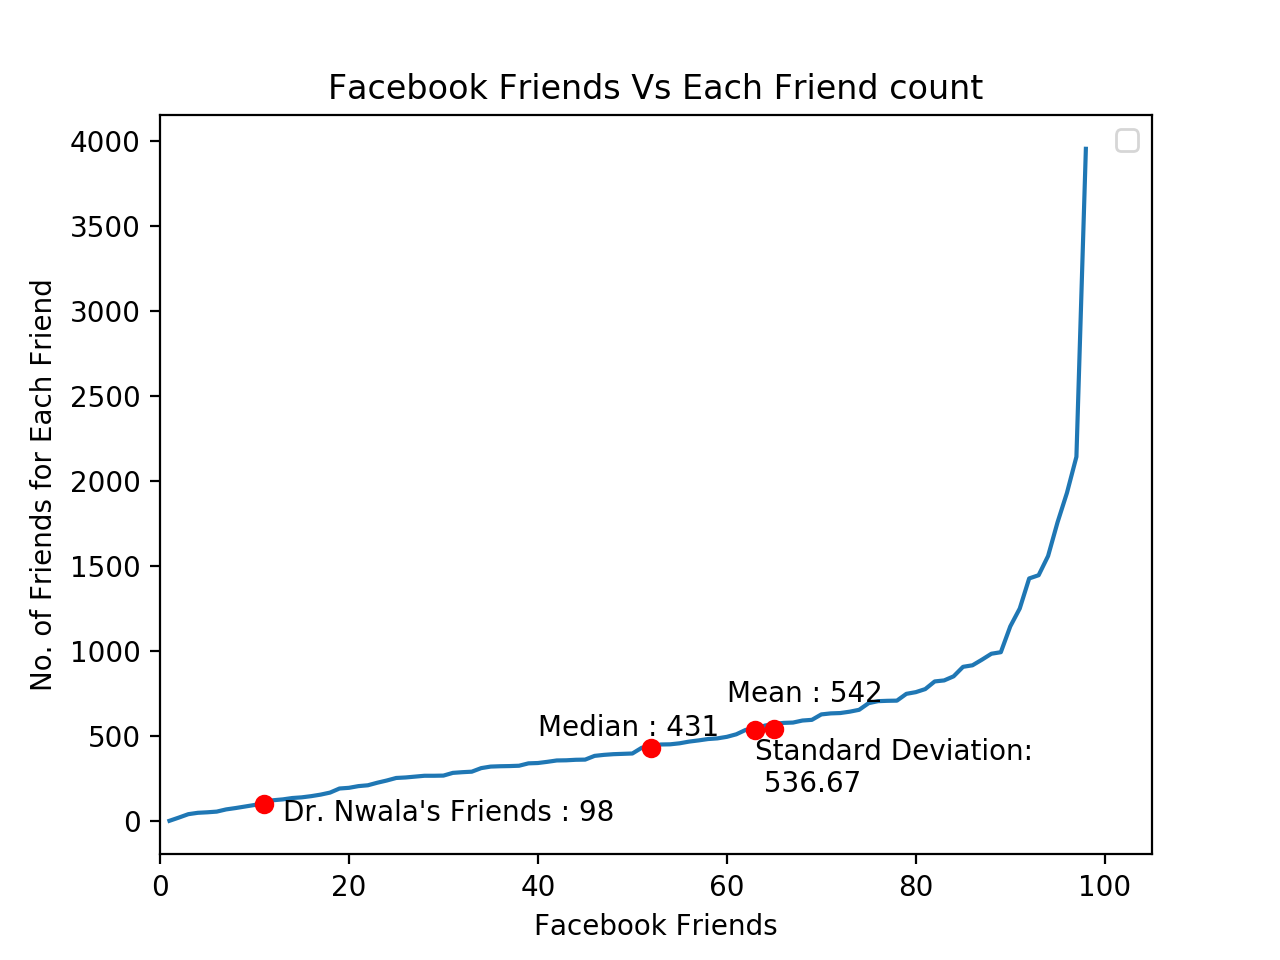
\includegraphics[width=0.8\textwidth]{Figure1}
      \caption{Friends vs Friends Count (Facebook) }
	\end{figure}

\end{homeworkProblem}
\clearpage
\newpage

%----------------------------------------------------------------------------------------
%   PROBLEM 2
%----------------------------------------------------------------------------------------

\begin{homeworkProblem}
Determine if the friendship paradox holds for your Twitter account. Since Twitter is a directed graph, use "followers" as value you measure 
(i.e., "do your followers have more followers than you?")..\\
Generate the same graph as in question number 1, and calculate the same  mean, standard deviation, and median values..\\\\
%\problemAnswer{

 \textbf{SOLUTION}\\\\
 The program requires to use the access tokens generated while creating the twitter developer account . \\ 
 \begin{enumerate}
   	\item \textbf{} Download and install the twitter API i.e. \textbf{tweepy} : 
  			\begin{verbatim}
				pip install tweepy
			\end{verbatim}
			
			
	\item \textbf{} Currently running the tweepy on the \textbf{acnwala} twitter handle:
  	        		\begin{verbatim}
				user = tweepy.Cursor(api.followers, screen_name=twitter_handle, 
				count=200).items()
			\end{verbatim}
			The above statement will fetch all the followers details in JSON for the twitter handle.		      
 \end{enumerate}
 
\begin{lstlisting}[language=Python, caption=Assignment4_2.py]
 #This is a Python2 Program 
 
import tweepy
import time
import csv
import math
from astropy.table import Table

#My twitter Account keys
ckey = 'mtDSeNYtJUZkKfspxTFmk7Nn8'
csecret = 'iYg5kksoIQKGsXVwGZ7bYpH0cFlxonNPg9hyhDKdGoP89bic6G'
atoken = '1094978973245812738-msYR1atvDnyfTTO46shWdnp5SIJcAA'
asecret = 'EMdqw7fA4IfkDYzKBqNQfoe5sAwz7dgCcRTWkpZOteUKd'
#Login Verifiavtion 
auth = tweepy.auth.OAuthHandler(ckey, csecret)
auth.set_access_token(atoken, asecret)
api = tweepy.API(auth,wait_on_rate_limit=True)
if(api.verify_credentials):
    print ('Logged in successfully')

total_count = 0
listDict = {}
twitter_handle='acnwala'
friend_Mean = 0
friend_Median = 0
friend_SD = 0
friend_List = []
count = 1
friend_count = 0


def mean():
    global friend_Mean
    friend_Mean = round((friend_count / total_count),2)
    return friend_Mean


def median():  
    global friend_Median 
    mid = 0 
    friend_List.sort(key=int)
    avg = len(friend_List) % 2
    if(avg == 0):
        mid = len(friend_List) / 2
        friend_Median = friend_List[mid]
    else:
        mid = len(friend_List) / 2
        mid = mid +1    
        friend_Median = friend_List[mid]
    return friend_Median


def SD():
    global friend_SD
    global friend_Mean
    stdDeviationSum = 0
    for num in friend_List:
        stdDeviationSum = stdDeviationSum + ((int(num) - int(friend_Mean)) 
        								*  (int(num) - int(friend_Mean)))
        # print('stdDeviationSum',stdDeviationSum)  
        friend_SD = round(math.sqrt(stdDeviationSum / total_count),2)
    return friend_SD

for follower in tweepy.Cursor(api.followers, screen_name=twitter_handle).items(): 
    total_count = total_count + 1
    listDict[follower.screen_name] = follower.friends_count
    friend_List.append(follower.friends_count)

friend_List.sort(key=int)
f = open('twitterFollowers-Friends.txt','w')
for friendCount in friend_List:
    f.write(str(count)+","+str(friendCount))
    f.write('\n')
    count = count + 1
    friend_count = friend_count + friendCount
f.close()    

mean = [str(mean())]
median = [str(median())]
SD = [str(SD())]
tableList = Table([mean, median, SD], names=('MEAN', 'MEDIAN', 'STANDARD DEVIATION'))
print (tableList)

	
\end{lstlisting} 
%}

\begin{lstlisting}[language=Python, caption=graph4_2.py]
 #This is a Python2 Program 
 
 import matplotlib.pyplot as plt
import csv

x = []
y = []

with open('twitterFollowers-Friends.txt','r') as csvfile:
    plots = csv.reader(csvfile, delimiter=',')
    for row in plots:
        x.append(int(row[0]))
        y.append(int(row[1]))

plt.plot(x,y)
plt.plot(65,250,marker='.', color='red',markersize=12)
plt.annotate('Dr.Nwala\'s Followers:250' , xy=(2, 620))

plt.plot(117,560,marker='.', color='red',markersize=12)
plt.annotate('Median:560' , xy=(120, 150))

plt.plot(185,1461.0,marker='.', color='red',markersize=12)
plt.annotate('Mean:1461.0' , xy=(190, 1260))


plt.plot(225, 3634.72,marker='.', color='red',markersize=12)
plt.annotate('Standard\nDeviation:3634.72' , xy=(140, 4000))

plt.xlim(0, 300)
plt.ylim(0, 10000)

plt.xlabel('All Followers')
plt.ylabel('No. of Friends for Each Follower')
plt.title('Twitter Followers Vs Each Follower\'s Friend count')
plt.legend()
plt.show()

\end{lstlisting}

The below plot will show the friendship paradox for \textbf{Dr.Alexander Nwala's}  twitter handle.

\begin{figure}[h]
  \centering
    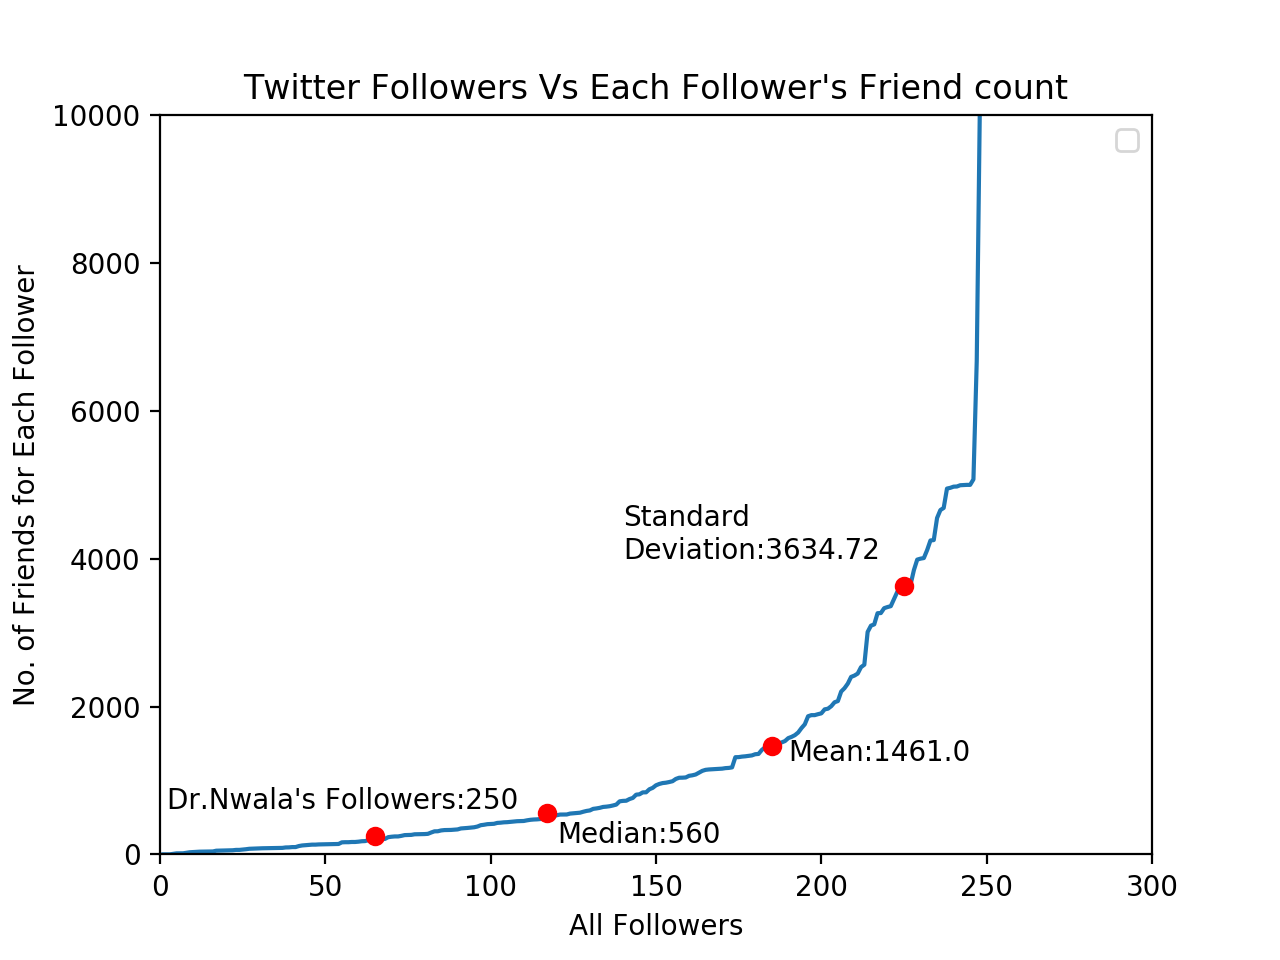
\includegraphics[width=0.8\textwidth]{Figure2}
      \caption{Followers vs Followers Count (Twitter) }
	\end{figure}


\newpage

The Sorted friend's list can be found in the \textbf{twitterFollowers-Friends.txt} text file.
 
\end{homeworkProblem}
\clearpage
\newpage

%----------------------------------------------------------------------------------------
%   PROBLEM 4
%----------------------------------------------------------------------------------------

\begin{homeworkProblem}
Repeat question number 2, but change "followers" to "following"?  In other words, are the people I am following following more people?\\

%\problemAnswer{
 \textbf{SOLUTION}\\\\
 The program requires to use the access tokens generated while creating the twitter developer account .
 \begin{enumerate}
   	
	\item \textbf{} Running the tweepy on the \textbf{acnwala} twitter handle:
  	        		\begin{verbatim}
				user = tweepy.Cursor(api.friends, screen_name=twitter_handle, 
				count=200).items()
			\end{verbatim}
			The above statement will fetch all the friends list in JSON for the twitter handle.		      
 \end{enumerate}
 

\begin{lstlisting}[language=Python, caption=AssignmentExC4_4.py]
#This is a Python2 Program 
import tweepy
import time
import csv
import math
from astropy.table import Table

#My twitter Account keys
ckey = 'mtDSeNYtJUZkKfspxTFmk7Nn8'
csecret = 'iYg5kksoIQKGsXVwGZ7bYpH0cFlxonNPg9hyhDKdGoP89bic6G'
atoken = '1094978973245812738-msYR1atvDnyfTTO46shWdnp5SIJcAA'
asecret = 'EMdqw7fA4IfkDYzKBqNQfoe5sAwz7dgCcRTWkpZOteUKd'
#Login Verifiavtion 
auth = tweepy.auth.OAuthHandler(ckey, csecret)
auth.set_access_token(atoken, asecret)
api = tweepy.API(auth,wait_on_rate_limit=True)
if(api.verify_credentials):
    print ('Logged in successfully')

total_count = 0
listDict = {}
twitter_handle='acnwala'
friend_Mean = 0
friend_Median = 0
friend_SD = 0
friend_List = []
count = 1
friend_count = 0


def mean():
    global friend_Mean
    friend_Mean = round((friend_count / total_count),2)
    return friend_Mean


def median():  
    global friend_Median 
    mid = 0 
    friend_List.sort(key=int)
    avg = len(friend_List) % 2
    if(avg == 0):
        mid = len(friend_List) / 2
        friend_Median = friend_List[mid]
    else:
        mid = len(friend_List) / 2
        mid = mid +1    
        friend_Median = friend_List[mid]
    return friend_Median


def SD():
    global friend_SD
    global friend_Mean
    stdDeviationSum = 0
    for num in friend_List:
        stdDeviationSum = stdDeviationSum + ((int(num) - int(friend_Mean)) 
        								*  (int(num) - int(friend_Mean)))
        # print('stdDeviationSum',stdDeviationSum)  
        friend_SD = round(math.sqrt(stdDeviationSum / total_count),2)
    return friend_SD

for follower in tweepy.Cursor(api.friends, screen_name=twitter_handle).items(): 
    total_count = total_count + 1
    listDict[follower.screen_name] = follower.friends_count
    friend_List.append(follower.friends_count)

friend_List.sort(key=int)
f = open('twitterFollowing.txt','w')
for friendCount in friend_List:
    f.write(str(count)+","+str(friendCount))
    f.write('\n')
    count = count + 1
    friend_count = friend_count + friendCount
f.close()    

mean = [str(mean())]
median = [str(median())]
SD = [str(SD())]
tableList = Table([mean, median, SD], names=('MEAN', 'MEDIAN', 'STANDARD DEVIATION'))
print (tableList)
\end{lstlisting}
   
\newpage
   
\begin{lstlisting}[language=Python, caption=graphExC4_4.py]
#This is a Python2 Program 
import matplotlib.pyplot as plt
import csv

x = []
y = []

with open('twitterFollowing.txt','r') as csvfile:
    plots = csv.reader(csvfile, delimiter=',')
    for row in plots:
        x.append(int(row[0]))
        y.append(int(row[1]))

plt.plot(x,y)
plt.plot(10,92,marker='.', color='red',markersize=12)
plt.annotate('Dr.Nwala\'s Friends: 92', xy=(1, 392))

plt.plot(43,461,marker='.', color='red',markersize=12)
plt.annotate('Median: 461' , xy=(42, 121))

plt.plot(73.5,1255,marker='.', color='red',markersize=12)

plt.annotate('Mean: 1255.0' , xy=(76, 1250.0))

plt.plot(81.5,2625,marker='.', color='red',markersize=12)
plt.annotate('Standard\nDeviation: 2625.42' , xy=(51, 2500.42))

plt.ylim(0, 7000)
plt.xlim(0, 100)

plt.xlabel('All Friends')
plt.ylabel('No. of Friends for Each Friend')
plt.title('Twitter Friends Vs Each Friend count')
plt.legend()
plt.show()



\end{lstlisting}

The below plot will show the friendship paradox for \textbf{Dr.Alexander Nwala's}  twitter handle.

\begin{figure}[h]
  \centering
    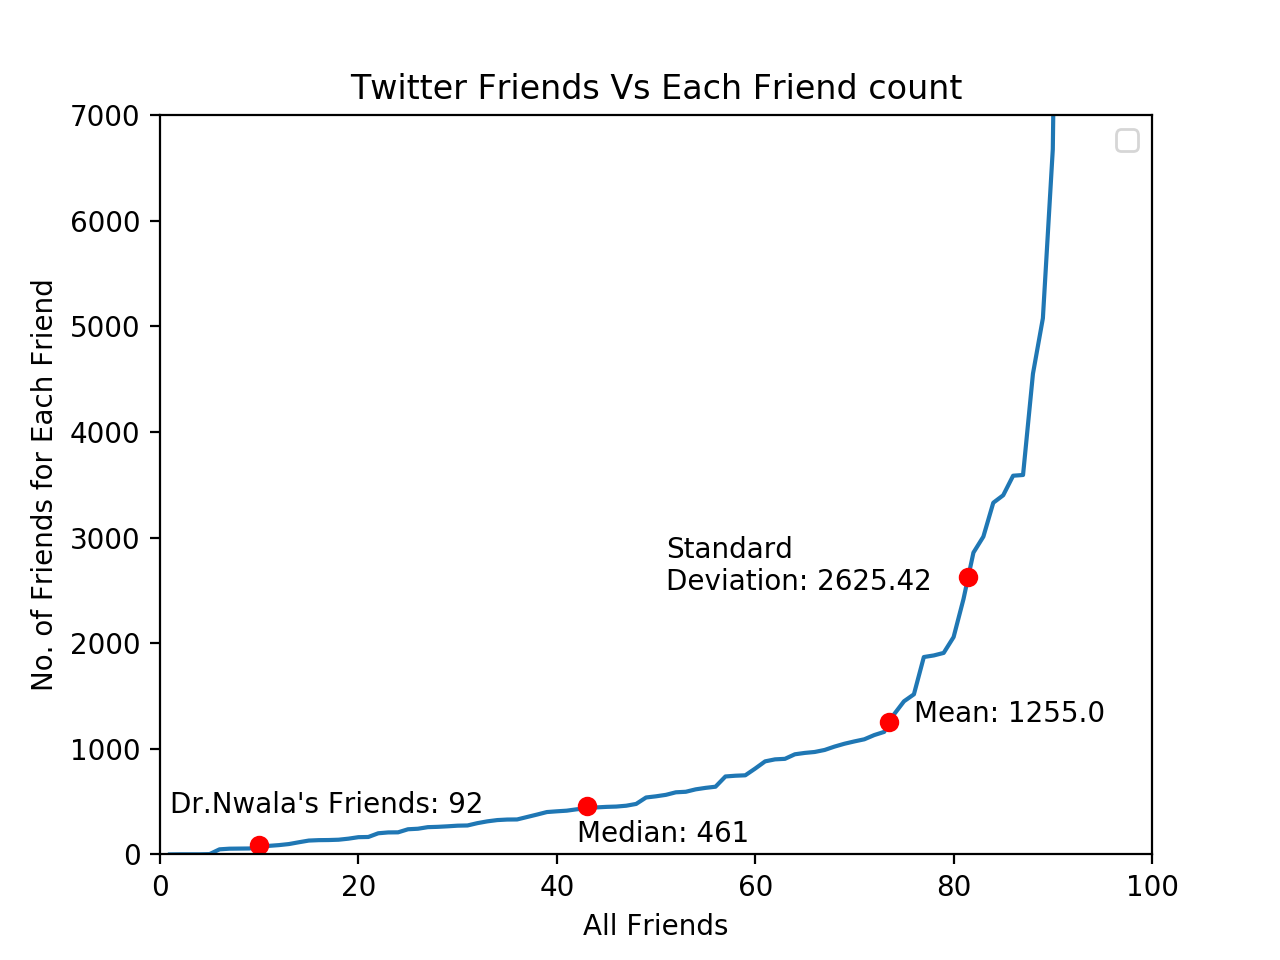
\includegraphics[width=0.8\textwidth]{graphExC}
      \caption{Following vs Following Count (Twitter) }
	\end{figure}   
\newpage
The Sorted friend's list can be found in the \textbf{twitterFollowing.txt} text file.
		
%}

\end{homeworkProblem}
\clearpage
\newpage

\bibliographystyle{plain}
\bibliography{A1bibFile}

\end{document}
